\documentclass{article}%
\usepackage[T1]{fontenc}%
\usepackage[utf8]{inputenc}%
\usepackage{lmodern}%
\usepackage{textcomp}%
\usepackage{lastpage}%
\usepackage[head=40pt,margin=0.5in,bottom=0.6in]{geometry}%
\usepackage{graphicx}%
%
\title{\textbf{Docentes de Vargas exigen pago de deudas pendientes}}%
\author{AMY TORRES}%
\date{04/10/2018}%
%
\begin{document}%
\normalsize%
\maketitle%
\textbf{URL: }%
http://www.eluniversal.com/caracas/22305/docentes{-}de{-}vargas{-}exigen{-}pago{-}de{-}deudas{-}pendientes\newline%
%
\textbf{Periodico: }%
EU, %
ID: %
22305, %
Seccion: %
caracas\newline%
%
\textbf{Palabras Claves: }%
NO\_TIENE\newline%
%
\textbf{Derecho: }%
2.3, %
Otros Derechos: %
, %
Sub Derechos: %
2.3.4\newline%
%
\textbf{EP: }%
SI\newline%
\newline%
%
\textbf{\textit{Según el profesor Santos Sivira, miembro de Sitravargas "todavía nos deben toda la homologación de la segunda convección colectiva del contrato único y unitario del Ministerio de Educación"}}%
\newline%
\newline%
%
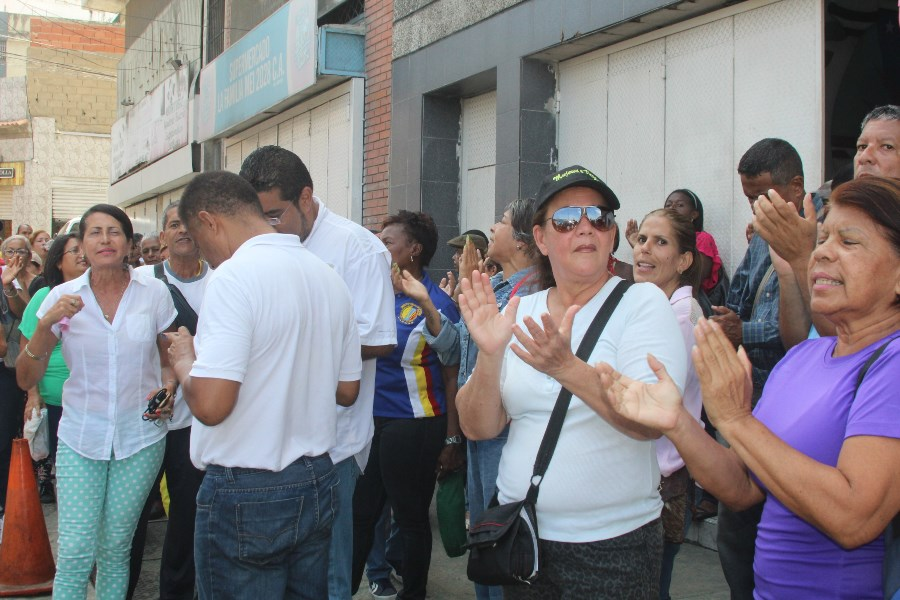
\includegraphics[width=300px]{200.jpg}%
\newline%
%
La Guaira.{-}~Más de 100 maestros, obreros, jubilados y personal administrativo adscritos a la Gobernación de Vargas sostuvieron una asamblea general en la Cámara de Comercio de La Guaira y luego acudieron a Manoa, sede de la Dirección de Administración del Ejecutivo regional para exigir respuestas.%
\newline%
%
"Reclaman la violación de los acuerdos por parte de la primera dama María de García y del profesor Rafael Bravo, comisionado de Educación, quienes prometieron que el último de agosto terminarían de cancelar las deudas pendientes y resulta que todavía nos deben toda la homologación de la segunda convección colectiva del contrato único y unitario del Ministerio de Educación", según el profesor Santos Sivira, miembro de Sitravargas.%
\newline%
%
Explicó que el personal docente está dispuesto a tomar las medidas necesarias para que respeten sus cláusulas y su contratación colectiva. Lamentó que con el nuevo sueldo soberano "el Presidente trituró todos los tabuladores de los funcionarios públicos. No es posible que un profesor con doctorado o especialista gane igual que un licenciado".%
\newline%
%
Criticó que la infraestructura escolar está por el suelo. "También hay docentes que no tienen cómo llegar a los planteles, que no tienen ropa ni zapatos, menos medicinas. Nos han desmejorado totalmente".Sostuvo que se les están violando todas las cláusulas contractuales "que a partir del 1 de octubre hay un aumento del 40\% y vienen una serie de aumentos que siguen en diciembre y luego en enero. En Vargas somos más de 4.500 los afectados".%
\newline%
%
\end{document}